
\documentclass[
12pt,
a4paper,
pdftex,
czech,
titlepage
]{report}

\usepackage[czech]{babel}
\usepackage[utf8]{inputenc}
\usepackage{lmodern}
\usepackage{textcomp}
\usepackage{verbatimbox}
\usepackage[T1]{fontenc}
\usepackage{amsfonts}
\usepackage{titlesec}
\usepackage{graphicx}
\usepackage[unicode]{hyperref}
\usepackage{wrapfig}
\usepackage{float}
\usepackage{caption}
\usepackage{listings}
\usepackage{subcaption}
\usepackage{tikz}
\usetikzlibrary{calc,shapes.multipart,chains,arrows}


\hypersetup{ colorlinks = true, linkcolor = black, urlcolor= black}

\titleformat{\chapter}
  {\normalfont\LARGE\bfseries}{\thechapter}{1em}{}
\titlespacing*{\chapter}{0pt}{0ex plus 1ex minus .2ex}{2.0ex plus .2ex}

\begin{document}

\begin{titlepage}
	\vspace*{-2cm}
	{\centering
\includegraphics[scale=1.0]{logo.pdf}\par}
	\centering
	\vspace*{2cm}
	{\Large Semestrální práce z KIV/UIR\par}
	\vspace{1.5cm}
	{\Huge\bfseries Klasifikace dokumentů\par}
	\vspace{2cm}

	{\Large Matěj Zeman\par}
	{\Large A18B0360P\par}
	{\Large zemanm98@students.zcu.cz\par}

	\vfill

	{\Large \today }
\end{titlepage}

\tableofcontents
\thispagestyle{empty}
\clearpage
%%%%%%%%%%%%%%%%%%%%%%%%%%%%%%%%%%%%%%%%%%%%%%%%%%%%%%%%%%%%%%%%
%       CHAPTER 1                         ZADÁNÍ
%%%%%%%%%%%%%%%%%%%%%%%%%%%%%%%%%%%%%%%%%%%%%%%%%%%%%%%%%%%%%%%
\chapter{Zadání}
\begin{itemize}
\item{Implementujte alesponň tři různé algoritmy (z prednášek i vlastní) pro tvorbu příznaků reprezentující textový dokument.}
\item{Implementujte alespoň dva různé klasifikační algoritmy (klasifikace s učitelem): 
\begin{itemize}
\item{Naivní Bayesův klasifikátor}
\item{Klasifikátor dle vlastní volby}
\end{itemize} } 
\item{Funkčnost programu bude následující:
\begin{itemize}
\item{spuštění s parametry:
\begin{itemize}
\item{\texttt{název\_klasifikátoru}}
\item{\textit{soubor\_se\_seznamem\_klasifikačních\_tříd}}
\item{\textit{trénovací\_množina}}
\item{\textit{testovací\_množina}}
\item{\textit{parametrizační\_algoritmus}}
\item{\textit{klasifikační\_algoritmus}}
\item{\textit{název\_modelu}}
\end{itemize} 
program natrénuje klasifikátor na dané trénovací množině, použije zadaný parametrizační a klasifikační algoritmus, zároveň vyhodnotí úspěšnost klasifikace a natrénovaný model uloží do souboru pro pozdější použití (např. s GUI).}
\item{spuštění s jedním parametrem:
\begin{itemize}
\item{\texttt{název\_klasifikátoru}}
\item{\textit{název\_modelu}}
\end{itemize}
ohodnoťte kvalitu klasifikátoru na dodaných datech, použijte metriku přesnost (accuracy), kde jako správnou klasifikaci uvažujte takovou, kde se klasifikovaná třída nachází mezi anotovanými. Otestujte všechny konfigurace klasifikátorů (tedy celkem 6 výsledků).}
\end{itemize} }
\end{itemize}


%%%%%%%%%%%%%%%%%%%%%%%%%%%%%%%%%%%%%%%%%%%%%%%%%%%%%%%%%%%%%%%%
%       CHAPTER 2                       Analýza úlohy
%%%%%%%%%%%%%%%%%%%%%%%%%%%%%%%%%%%%%%%%%%%%%%%%%%%%%%%%%%%%%%%
\chapter{Analýza úlohy}
Přirozený jazyk je velice těžko popsatelný formálně (např. matematickým aparátem), pokud bychom chtěli porozumět jakémukoliv textu, museli bychom vytvořit systém, který by dokázal textu porozumět stejně jako člověk, tedy porozumět i kontextu ve větě a vztahům mezi jednotlivými větami.

Cílem této semestrální práce je klasifikovat dokument do jedné z klasifikačních tříd. K tomu budeme muset implementovat nějaký vektorový model, který převede text do vektoru používaného v klasifikačních algoritmech.
\section{Struktura souborů}
Pro správný běh programu potřebujeme trénovací a testovací data s určitou strukturou. Testovací i trénovací dokumenty mají vždy dva řádky. Na prvním řádku jsou uvedeny již předem určené klasifikační třídy do kterých byl dokument zažazen. Na druhém řádku je pak obsah dokumentu, tedy text který se má klasifikovat (v případě testrovacích dat), nebo se z něj mají tvořit slovníky pro klasifikační třídy (v případě trénovacích dat).
\section{Příznakové algoritmy}
V semestrální práci bylo potřeba použít tři příznakové algoritmy. Já se rozhodl pro následující:
\begin{itemize}
\item{\textbf{N-Gram}
\begin{itemize}
\item{Tato příznaková metoda vytváří z předaného textu slovník s výskyty jednotlivých segmentů textu. V semestrální práci jsem použil bi-gram, tedy ve slovnících jsou uloženy dvojice slov a jejich četnost. Metoda se tedy pokouší vzít v úvahu i kontext jednotlivých slov. Na trénovací množině souborů se pro každou klasifikační třídu vytvoří její slovník, který obsahuje prvky o dvou slovech a jejich četnost v dané klasifikační třídě.}
\end{itemize}}
\item{\textbf{Bag of Words}
\begin{itemize}
\item{Často používaná příznaková metoda, která je snadná na implementaci. Jedná se v podstatě o \texttt{N-Gram}, ale pouze po jednom slovu. Každá klasifikační třída má tedy slovník, kde v každém prvku je pouze jedno slovo a jeho četnost. Tato metoda nebere v potaz kontext slov, ale pouze výskyt unikátních slov ve třídách.}
\end{itemize}}
\item{\textbf{TF-IDF}
\begin{itemize}
\item{Tento model řeší problém s vysokou četností bezvýznamových slov. V češtině se objevuje mnoho bezvýznamových slov (např.:'a', 'se', 'po' atd.). Algoritmus TF-IDF narozdíl od ostatních metoda dává větší váhu slovům, která mají malou četnost (nadhodnotí je) a slovům s vysokou četností váhu sníží (podhodnotí je). Slova která jsou více charakteristická pro některou ze tříd tedy vezme s větší váhou.}
\end{itemize}}
\end{itemize}

\section{Klasifikační algoritmy}
Klasifikační algoritmy mají za úkol rozhodnout o předaném textu do které z klasifikačních tříd patří. K tomu potřebují natrénovaná data, tedy připravené slovníky klasifikačních tříd. V semestrální práci jsou naimplementované následující algoritmy:
\begin{itemize}
\item{\textbf{Naivní Bayesův klasifikátor}
\begin{itemize}
\item{Tento klasifikátor používá ke klasifikaci pravděpodobnosti. Pro každé slovo ze vstupní množiny spočítá pravděpodobnost jeho příslušnosti do jednotlivých klasifikačních tříd. Jednotlivé pravděpodobnosti poté vynásobí a dostane výslednou pravděpodobnost příslušnosti celého dokumentu do jedné ze tříd. Bylo ovšem třeba vyřešit problém, když se slovo v dané klasifikační třídě neobjevilo, tedy jedna z násobených pravděpodoností by byla nulová a tudíž i celá pravděpodobnost by byla rovna nule, bylo třeba použít \texttt{Laplace smoothing} metodu. Pravděpodobnost pro jednotlivá slova předaného textu se tedy počítá následovně: \textit{(počet výskytů slova ve třídě + 1)/(počet všech slov ve třídě + počet všech slov v trénovacích datech)}. Takto vypočítané pravděpodobnosti byly ovšem příliš malé a proto je bylo třeba logaritmovat a místo násobení sčítat. Tímto způsobem byla spočítána pravděpobnost příslušnosti dokumentu do jednotlivých klasifikačních tříd.} 
\end{itemize}}
\item{\textbf{Klasifikátor s nejmenší vzdáleností}
\begin{itemize}
\item{Tento klasifikátor používá ke klasifikaci vzdálenosti mezi dokumentem a klasifikačními třídami. Pro každé slovo spočítá vzdálenost od stejného slova v jednotlivých klasifikačních třídách (pokud se v nich vyskytuje) pomocí Manhattanské metriky. Četnost slova v klasifikovaném dokumentu se odečte od četnosti slova v dané klasifikační třídě a absolutní hodnota tohoto výpočtu je brána jako vzdálenost tohoto slova od klasifikační třídy. Jednotlivé vzdálenosti se pro každou klasifikační třídu sečtou a vydělí počtem společných slov s klasifikovaným dokumentem.}
\end{itemize}}
\end{itemize}

\chapter{Implementace}
Semestrální práce byla napsána v jazyce Python (verze 3.6). V rámci semestrální práce byla použita pouze knihovny:
\begin{itemize}
\item{\texttt{re} - pro práci s regulárními výrazy při dělení a filtrování textu.}
\item{\texttt{unidecode} - opět pro lepší zpracování textu.}
\item{\texttt{math} - pro logaritmování v Naivním Bayesovo klasifikátoru.}
\item{\texttt{json} - pro snadné ukládání modelu do souboru.}
\item{\texttt{sys} - pro práci se vstupními argumenty.}
\item{\texttt{tkinter} - pro vytváření a práci s GUI programu.}
\end{itemize}

\section{Třídy}
Jak již bylo řečeno výše, program má tři algoritmy pro tvorbu příznaků a dva klasifikační. Všechny algoritmy jsou rozděleny do svých tříd.
\begin{itemize}
\item{\textbf{Main.py}
\begin{itemize}
\item{Tato třída zajišťuje kontrolu vstupních argumentů a na jejich základě pak spustí jeden z typů běhu programu. Dále jsou zde metody pro GUI programu}
\end{itemize}}
\item{\textbf{BagOfWords.py}
\begin{itemize}
\item{Třída představuje příznakovou metodu \texttt{Bag of words}. Dostane množinu trénovacích souborů a množinu klasifikačních tříd. Třída obsahuje metody pro filtraci a rozdělení textu na jednotlivá slova.  Pro každou klasifikační třídu vytvoří její slovník, tedy jednotlivá slova a jejich četnost.}
\end{itemize}}
\item{\textbf{Tfidf.py}
\begin{itemize}
\item{Třída představuje příznakovou metodu \texttt{TF-IDF}. Stejně jako třída \texttt{BagOfWords.py} rozdělí trénovací množinu do slovníků pro jednotlivé klasifikační třídy, ale ještě nadhodnotí málo frekventovaná slova a podhodnotí ta často se vyskytující.}
\end{itemize}}
\item{\textbf{NGram.py}
\begin{itemize}
\item{Třída představuje příznakovou metodu \texttt{N-Gram}. Chová se velmi podobně jako třída \texttt{BagOfWords.py}, ale slova ve slovnících rozdělí na dvojice a spočte jejich četnosti v trénovací množině.}
\end{itemize}}
\item{\textbf{NaiveBayes.py}
\begin{itemize}
\item{Třída představuje Naivní Bayesův klasifikátor. Třída dostane jako parametr příznakovou metodu, tedy všechny klasifikační třídy a jejich slovníky a množinu s testovacími soubory. Každý soubor rozdělí pomocí metody \textit{tokenize} na jednotlivá slova a spočtě jejich pravděpodobnost zařazení do jednotlivých klasifikačních tříd. Poté jednotlivé pravděpodobnosti zlogaritmuje a sečte. Nejpravděpodobnější klasifikační třídy pak vypíše do konzole}
\end{itemize}}
\item{\textbf{NN.py}
\begin{itemize}
\item{Třída představuje Klasifikátor s nejmenší vzdáleností. Parametry dostane stejné jako třída \texttt{NaiveBayes.py} a stejně i rozdělí text. Klasifikace jako taková je ovšem rozdílná. Klasifikátor pro jednotlivá slova z dokumentu spočítá jejich vzdálenost pomocí Manhattanské metriky ke klasifikačním třídám. Jednotlivé vzdálenosti sečte a vydělí počtem společných slov. Poté opět vybere nejpravděpodobnější třídy a vypíše je do konzole.}
\end{itemize}}
\end{itemize}

%%%%%%%%%%%%%%%%%%%%%%%%%%%%%%%%%%%%%%%%%%%%%%%%%%%%%%%%%%%%%%%%
%       CHAPTER 4                    Adresářová struktura
%%%%%%%%%%%%%%%%%%%%%%%%%%%%%%%%%%%%%%%%%%%%%%%%%%%%%%%%%%%%%%%




%%%%%%%%%%%%%%%%%%%%%%%%%%%%%%%%%%%%%%%%%%%%%%%%%%%%%%%%%%%%%%%%
%       CHAPTER 5                      Uživatelská příručka
%%%%%%%%%%%%%%%%%%%%%%%%%%%%%%%%%%%%%%%%%%%%%%%%%%%%%%%%%%%%%%%
\chapter{Uživatelská příručka}
Program lze spustit ve dvěma způsoby:
\begin{itemize}
\item{Spuštění se sedmi parametry:
\begin{figure}[h]
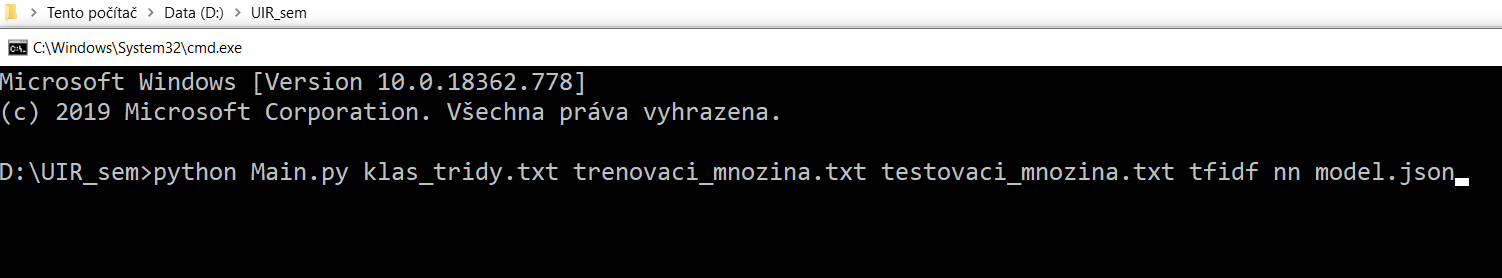
\includegraphics[width=13cm]{obr1.png}
\caption{Příklad spuštění programu se sedmi parametry.}
\label{obr1}
\end{figure}
\begin{itemize}
\item{\textit{Main.py} - argument určuje hlavní modul programu který se má spustit (vždy bude Main.py).}
\item{\textit{klas\_tridy.txt} - soubor obsahující názvy všech klasifikačních tříd do kterých se mají dokumenty zařazovat.}
\item{\textit{trenovaci\_mnozina.txt} - soubor obsahující cesty ke trénovacím dokumentům pro klasifikátor. Tyto dokumenty jsou potřeba pro slovníky klasifikačních tříd.}
\item{\textit{testovaci\_mnozina.txt} - soubor obsahující cesty k dokumentům které se mají klasifikovat.}
\item{\textit{tfidf} - příklad příznakové metody, která se v programu má použít. Další možnosti jsou:
\begin{itemize}
\item{\textit{ngram} - program použije k tvorbě příznaků algoritmus \texttt{N-Gram}}
\item{\textit{bow} - program použije k tvorbě příznaků algoritmus \texttt{Bag Of Words}}
\end{itemize}}
\item{\textit{nn} - příklad klasifikačního algoritmu, který se má v programu použít. Další možnost je:
\begin{itemize}
\item{\textit{bayes} - program použije pro klasifikaci Naivní Bayesův klasifikátor.}
\end{itemize}
}
\item{\textit{model.json} - určuje název soubpru do kterého se má model uložit pro další spuštění.}
\end{itemize}
\pagebreak
}
\item{Spuštění se dvěma parametry:
\begin{figure}[h]
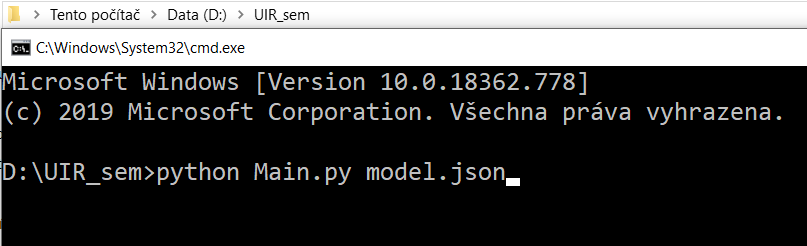
\includegraphics[width=13cm]{obr2.png}
\caption{Příklad spuštění programu se dvěma parametry.}
\label{obr1}
\end{figure}
\begin{itemize}
\item{\textit{Main.py} - argument určuje hlavní modul programu který se má spustit (vždy bude Main.py).}
\item{\textit{model.json} - json soubor ze kterého se má načíst model pro klasifikaci.}
\end{itemize}
}
\end{itemize}

%%%%%%%%%%%%%%%%%%%%%%%%%%%%%%%%%%%%%%%%%%%%%%%%%%%%%%%%%%%%%%%%
%       CHAPTER 6                       Závěr
%%%%%%%%%%%%%%%%%%%%%%%%%%%%%%%%%%%%%%%%%%%%%%%%%%%%%%%%%%%%%%%
\chapter{Závěr}
V rámci aplikace jsem implementoval příznakové algoritmy \textit{Bag Of Words}, \textit{N-Gram} a \textit{TF-IDF}. Jako klasifikační algoritmy jsem použil \textit{Naivní Bayesův klasifikátor} a \textit{Klasifikátor s nejmenší vzdáleností}. Pro trénování bylo použito 412 dokumentů a testovaných bylo 99 dokumentů. 

V trénovacích datech byl ovšem nepoměr jednotlivých kategorií. Třetina trénovací množiny byla zařazena do klasifikační třídy reklama (rek) a pětina do třídy finančnictví a obchod (fin), proto mohou být výsledky trochu nepřesné a klasifikování zadané věty při spuštění s dvěma parametry také. Z následující tabulky lze vyčíst přesnost jednotlibých klasifikátorů a příznakových metod v nich použitých:
\begin{table}[h!]  
\begin{center}  
\caption{Tabulka přesností}  
\label{tab:Table1}  
\begin{tabular}{|l|c|r|}  
\textbf{Klasifikátor} & \textbf{Příznaková metoda} & \textbf{Přesnost}\\
\hline  
Naive Bayes & N-Gram & 15.5\% \\  
Naive Bayes & TF-IDF & 20.5\% \\  
Naive Bayes & Bag Of Words & 33.7\% \\  
NN & N-Gram & 37.3\% \\  
NN & TF-IDF & 51.5\% \\  
NN & Bag Of Words & 33.3\% \\  
\end{tabular}  
\end{center}  
\end{table}  
Z výsledků můžeme usoudit, že klasifikátor s nejbližsí vzdáleností je celkově přesnější a nejlépe klasifikuje ve spojení s příznakovým algoritmem TF-IDF. Naivní Bayesův klasifikátor zas nejlépe pracuje s příznakovou metodou Bag of words.
\end{document}